% RPG fantasy adventure.
% View with pdflatex sliapa_vrana.tex && evince sliapa_vrana.pdf.
% sir.vorac@gmail.com

\documentclass{article}
\usepackage[T2A]{fontenc}
\usepackage[pdftex]{graphicx}
\usepackage[utf8]{inputenc}
\usepackage[bulgarian]{babel}
%\usepackage{iwona}
%\newenvironment{directspeech}{\itshape}{}
\newcommand{\directspeech}[1]{#1}  % TODO: make this italics.
\begin{document}
{\huge Сляпа врана}
\section{Кеделке}
Тук става дума за еволюция и креативизъм.
\section{Тези които ядат трупове}
%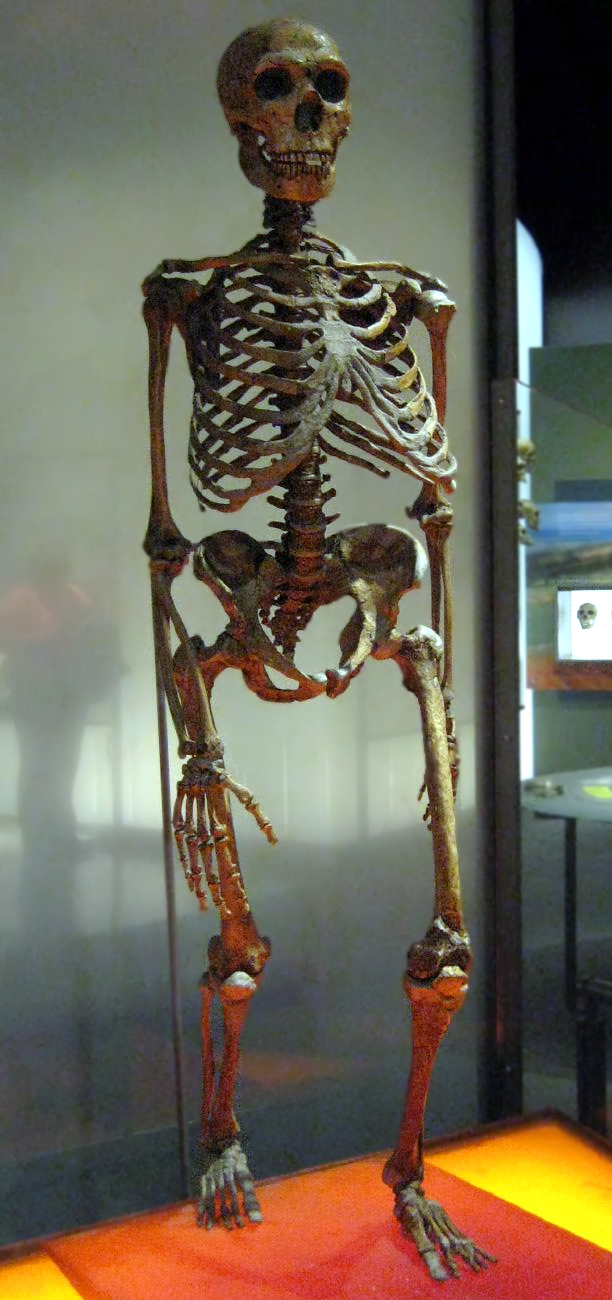
\includegraphics[height=0.25\textheight]{neanderthal1}
%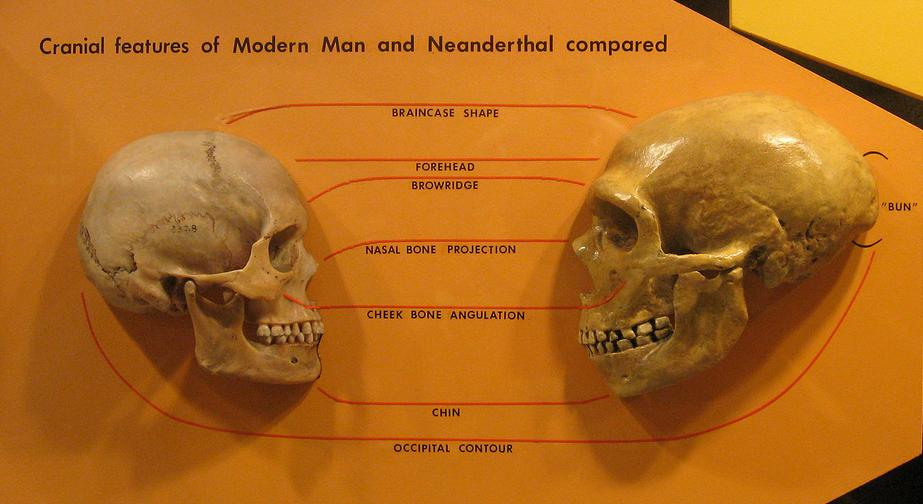
\includegraphics[height=0.25\textheight]{neanderthal2}


% Notes on the Burch Christian invasion.
% Leader: Saint Gatrem

\section{}
Това е разказ за креационизъм, история и еволюция.

Становището й е че боговете поставят видове в света през големи интервали от време.
Тези видове се изменят с времето, защото така е заложено при създаването им.


"Аз съм и креационист, и еволюционист.
Еволюцията е начина, по който Бог, или природата, твори.
Сътворението не е явление, случило се в 4004 г. пр. н. е.
То е процес, започнал преди около 10 милиарда години, който продължава и до днес...
Дали еволюционното учение е в разрез с религиозната вяра?
Не.
Глупава грешка е да се бърка Свещеното писание с елементарен учебник по астрономия, геология, биология и антропология.
Само ако символите биват тълкувани по начин, по който ще означават нещо, което те не са предвидени да означават, могат да възникнат въображаеми и неразрешими конфликти.
Глупавата грешка тогава се превръща в богохулство: Създателят бива обвинен в системна лъжа."
 Теодосиус Добжански (1900 – 1975)
\end{document}
